要想在数字音频设备之间进行通信,可以使用I2S同步串行通信协议。

在ESP32中,有实现I2S协议的库:\href{https://github.com/schreibfaul1/ESP32-audioI2S}{\underline{https://github.com/schreibfaul1/ESP32-audioI2S}}

首先要进行语音识别的实现,我选择使用INMP441 MEMS全向麦克风进行实时录音。
接下来聚焦的痛点是:如何将录音数据传输到LLM中进行语音识别?

幸运的是,讯飞开放平台中提供了流式语音识别的API,可以将录音数据实时传输到LLM中进行语音识别。
\textbf{以下,我们将语音转文字(Speech To Text)简写为STT,文字转语音(Text To Speech)简写为TTS}。
下一步即调用API接口,进入官方文档中获取相关的参数。

\begin{figure} [H]
    \centering
    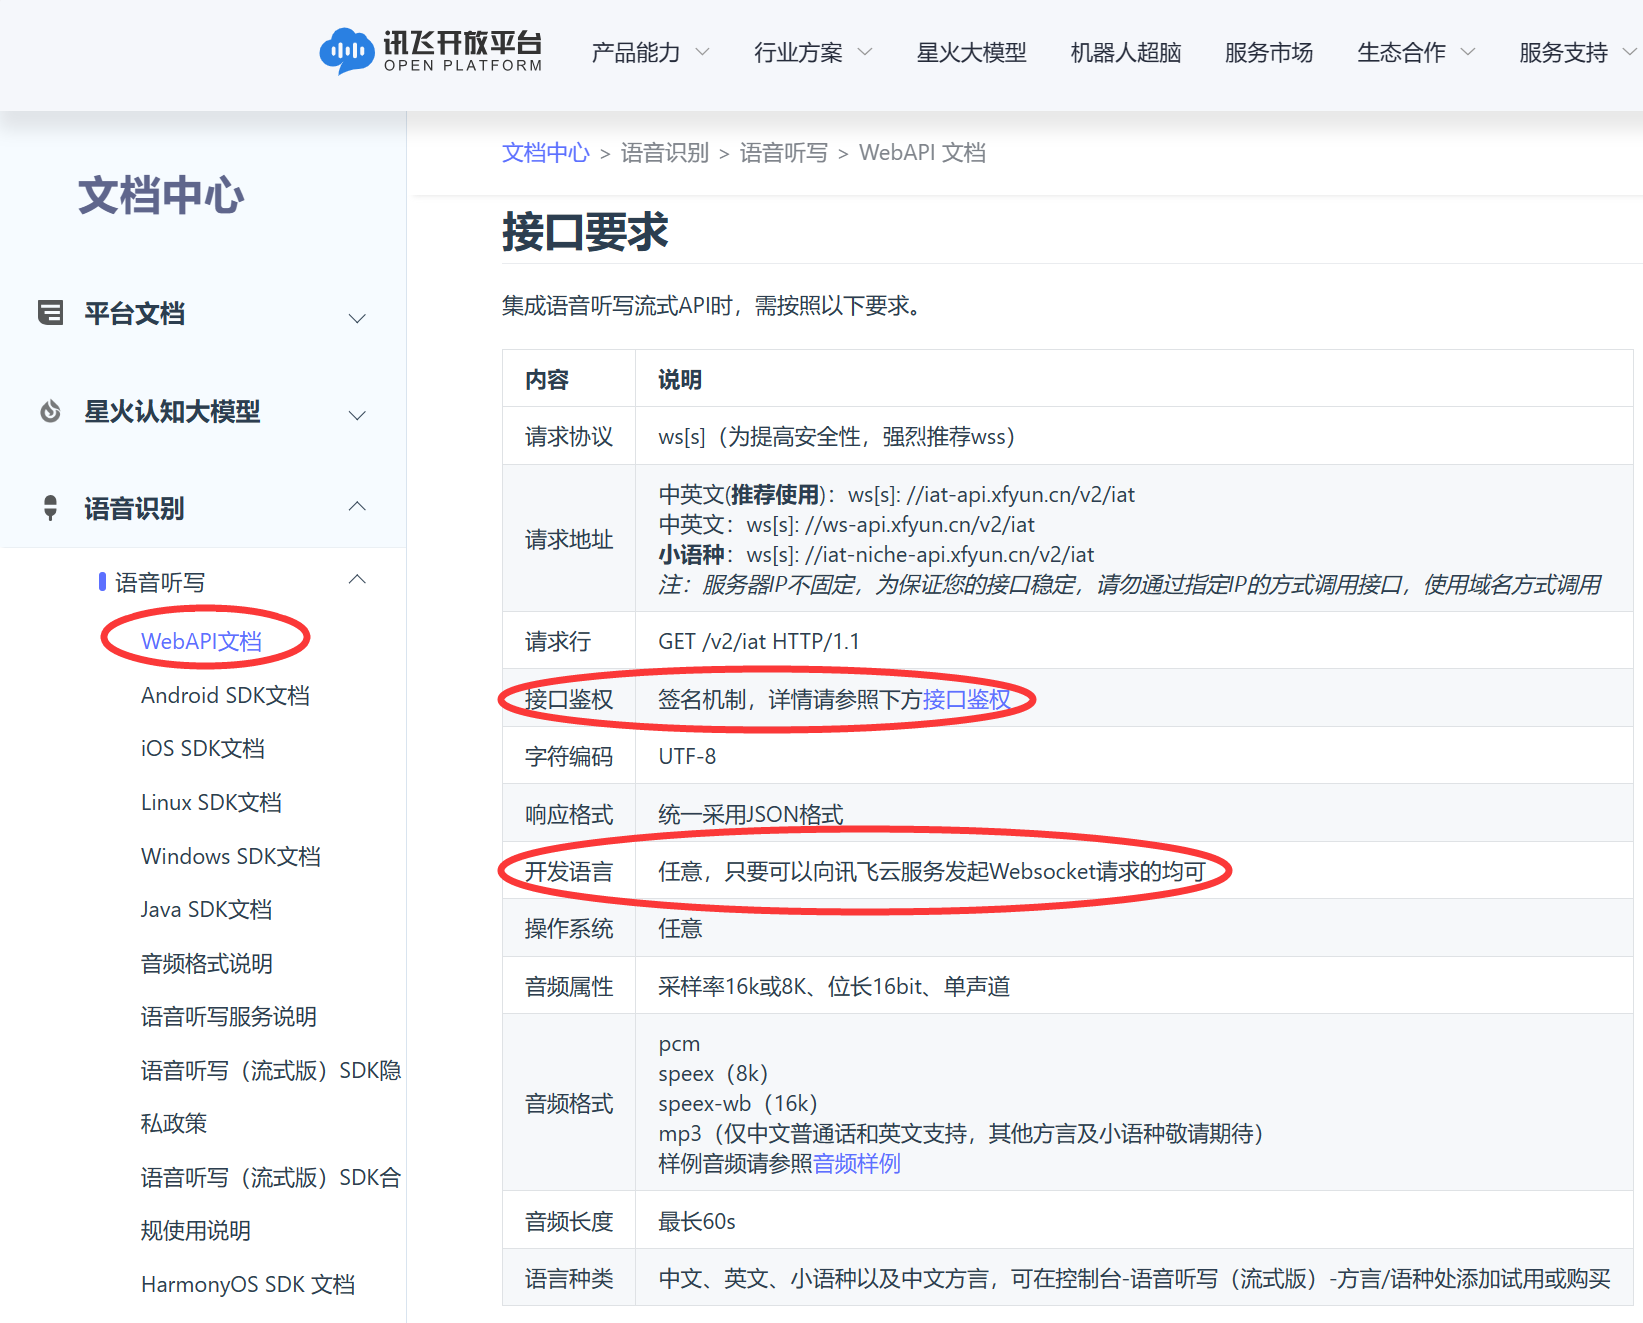
\includegraphics[width=0.53\textwidth]{../img/STTAPI.png}
    \caption{STT API接口参数列表}
    \label{fig:STTAPI}
\end{figure}

在调用接口时,需要按照下方所示的Url鉴权方法进行请求地址加鉴权参数的形式鉴权。

\begin{figure} [H]
    \centering
    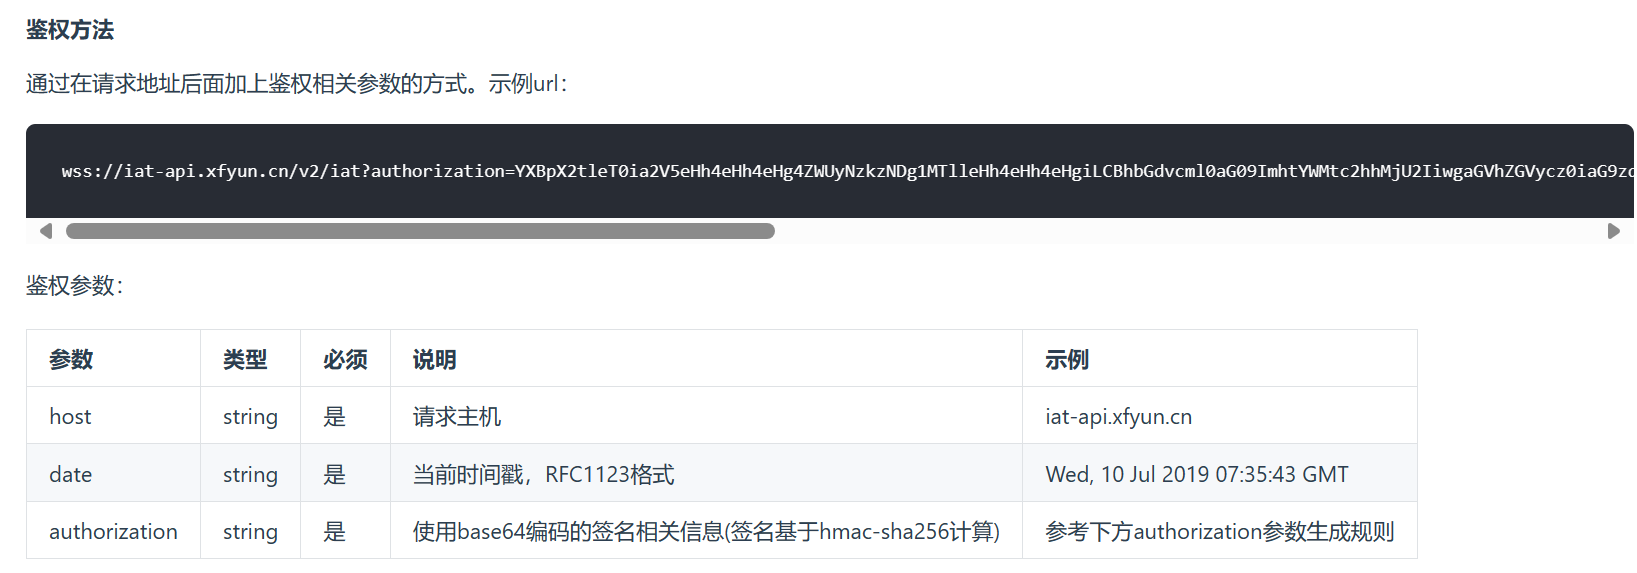
\includegraphics[width=0.6\textwidth]{../img/GetUrl.png}
    \caption{Url鉴权方法}
    \label{fig:Url Authorization}
\end{figure}

以下分别按照步骤进行鉴权:

\subsubsection{通过HTTP请求返回RFC 1123格式的时间戳}

\begin{lstlisting}[language = C++, title = {通过HTTP请求返回RFC1123格式的时间戳}]
void getRFC1123Time() {
    HTTPClient http;
    http.begin("https://www.baidu.com");

    // 从 HTTP 响应头中获取Date
    const char *headerKeys[] = {"Date"};
    http.collectHeaders(headerKeys, sizeof(headerKeys) / sizeof(headerKeys[0]));
    int httpCode = http.GET() ; // 必须要先设置收集字段,再发送HTTP请求,否则收集不到
    Date = http.header("Date");
    http.end();

    // Debug
    Serial.println("Date:" + Date);
    Serial.println("httpCode:" + httpCode);
}
\end{lstlisting}

\subsubsection{通过Hmac-sha256算法生成鉴权参数}

Hmac-sha256算法介绍部分见附件。此处我使用mbedTLS开源加密库实现算法。

\begin{lstlisting} [language = C++, title = {通过Hmac-sha256算法生成鉴权参数}]
String getOriginalSignature(String host, String date, String path) {
    return "host: " + host + "\n" + "date: " + date + "\n" + "GET " + path + " HTTP/1.1";
}

String getUrl(String Spark_url, String host, String path, String date) {
    String originalSignature = getOriginalSignature(host, date, path);
    const size_t originalSignatureLength = originalSignature.length(); // 原始签名的长度
    const size_t APIKeyLength = APISecret.length(); // API Key 的长度
    // 使用 HMAC-SHA256 进行加密
    unsigned char hmac[32]; // 存储HMAC结果
    mbedtls_md_context_t ctx; // HMAC上下文
    mbedtls_md_type_t md_type = MBEDTLS_MD_SHA256;
    mbedtls_md_init(&ctx);
    mbedtls_md_setup(&ctx, mbedtls_md_info_from_type(md_type), 1);
    mbedtls_md_hmac_starts(&ctx, (const unsigned char *) APISecret.c_str(), APIKeyLength);
    mbedtls_md_hmac_update(&ctx, (const unsigned char *) originalSignature.c_str(), originalSignatureLength);
    mbedtls_md_hmac_finish(&ctx, hmac);
    mbedtls_md_free(&ctx);

    // 将HMAC结果进行Base64编码
    String signature_sha_base64 = base64::encode(hmac, sizeof(hmac) / sizeof(hmac[0]));

    // 替换Date字符串中的特殊字符
    date.replace(",", "%2C");
    date.replace(" ", "+");
    date.replace(":", "%3A");

    // 构建Authorization原始字符串
    String authorization_origin = "api_key=\"" + APIKey + "\", algorithm=\"hmac-sha256\", headers=\"host date request-line\", signature=\"" + signature_sha_base64 + "\"";

    // 将Authorization原始字符串进行Base64编码
    String authorization = base64::encode(authorization_origin);

    // 构建最终的URL
    String FinalUrl = Spark_url + '?' + "authorization=" + authorization + "&date=" + date + "&host=" + host;
    Serial.println(FinalUrl); // Debug
    return FinalUrl;
}
\end{lstlisting}

鉴权完毕,在串口调试助手中返回了正确的鉴权Url:

\begin{figure} [H]
    \centering
    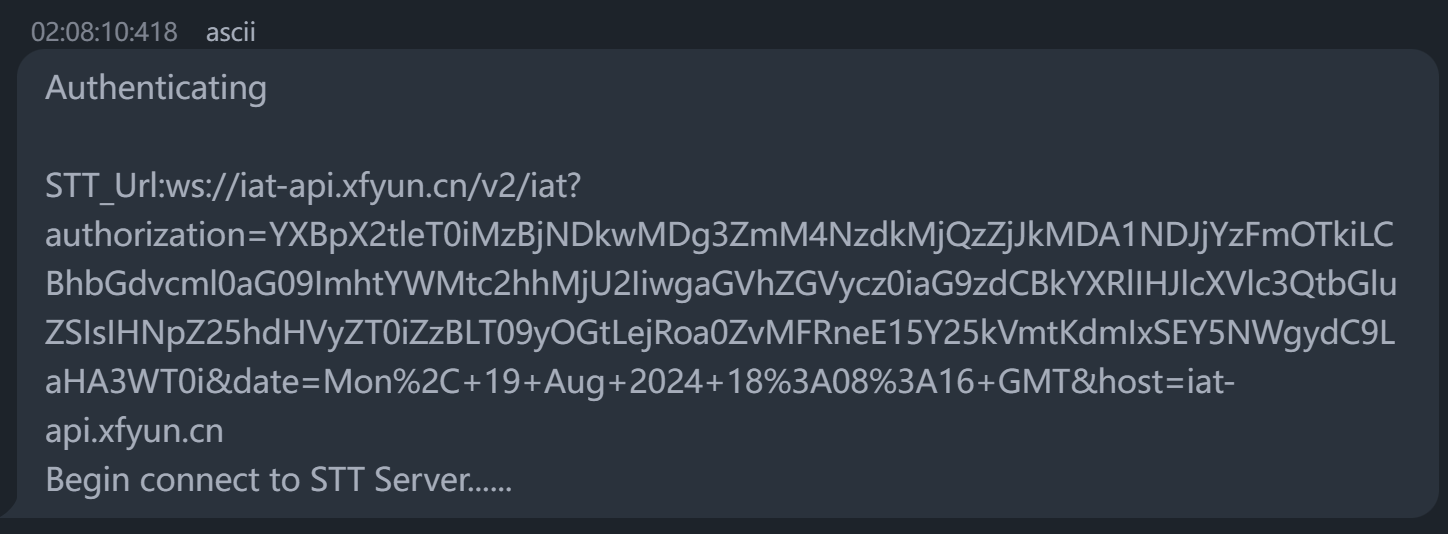
\includegraphics[width=0.4\textwidth]{../img/AuthSuccess.png}
    \caption{鉴权Url}
    \label{fig:AuthorizationUrl}
\end{figure}

\subsubsection{调用LLM API接口进行联网对话}

官方文档中所示示例如下,使用DynamicJson创建动态Json对象,按顺序构造Json即可。

\begin{figure} [H]
    \centering
    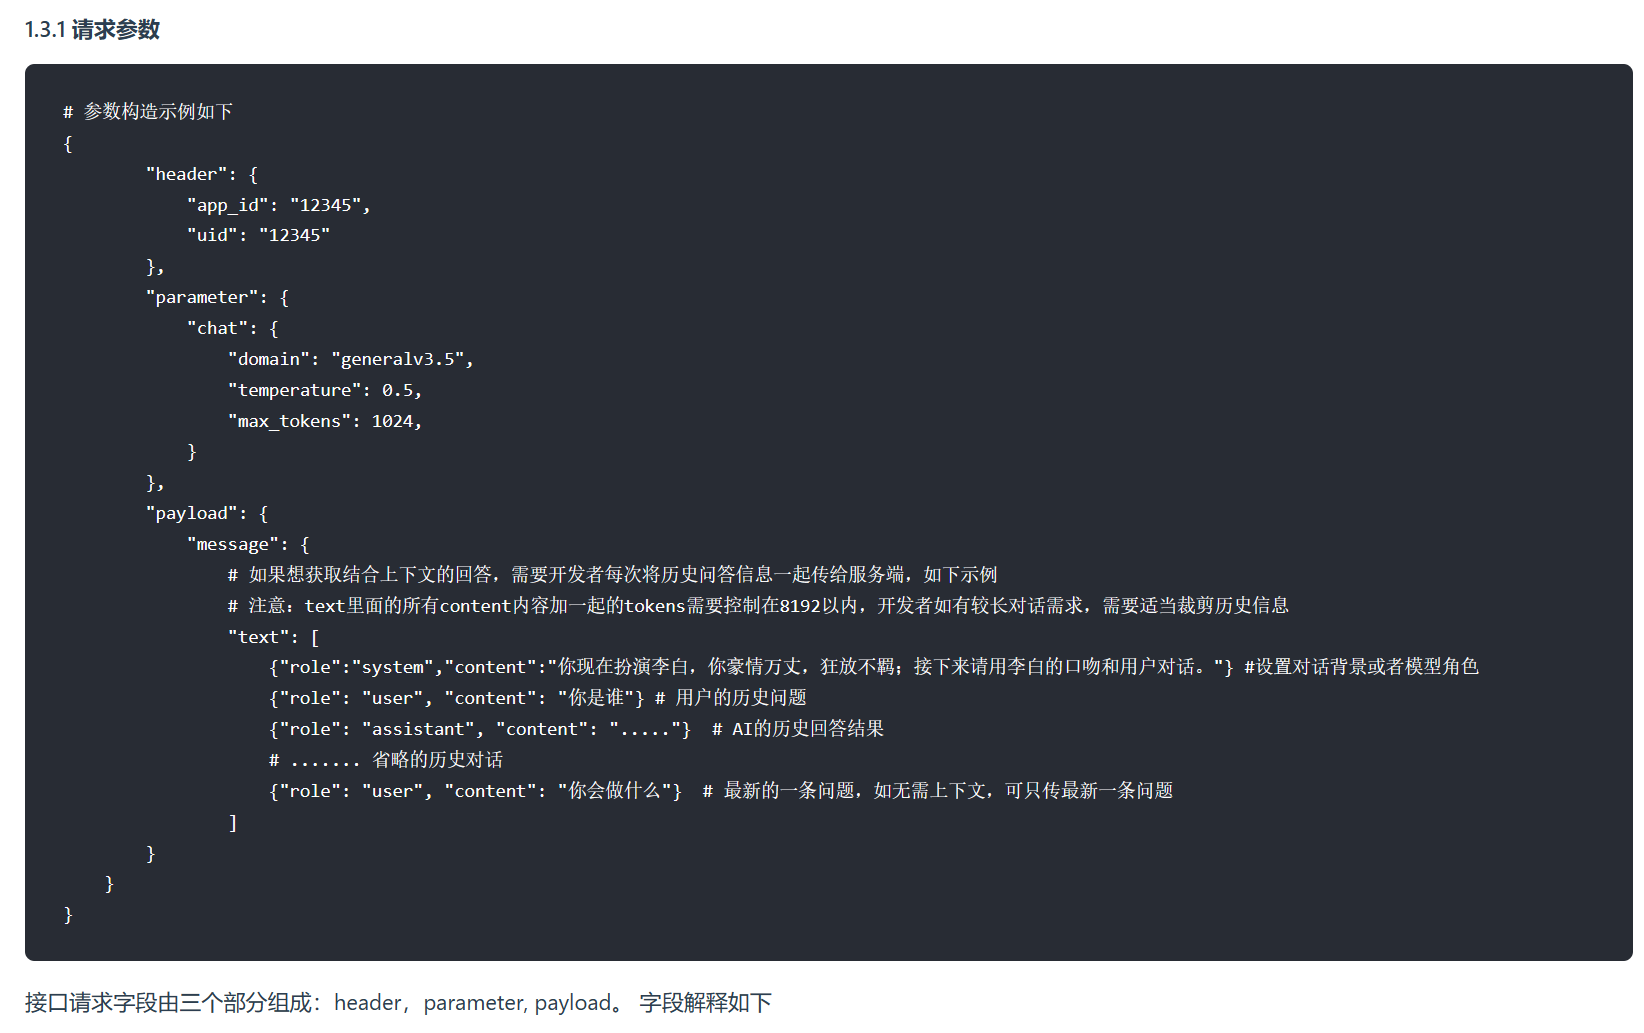
\includegraphics[width=0.6\textwidth]{../img/LLMAPI.png}
    \caption{LLM API参数构造}
    \label{fig:LLMAPI}
\end{figure}

\begin{lstlisting}[language = C++, title = {调用LLM API接口进行联网对话}]

DynamicJsonDocument getParameters(const char *appid, const char *domain, const char *role_set) {
    DynamicJsonDocument data(1500);
    // 构建Json的嵌套对象
    JsonObject header = data.createNestedObject("header");
    JsonObject parameter = data.createNestedObject("parameter");
    JsonObject chat = parameter.createNestedObject("chat");
    JsonObject payload = data.createNestedObject("payload");
    JsonObject message = payload.createNestedObject("message");
    JsonArray textArray = message.createNestedArray("text");
    JsonObject systemMessage = textArray.createNestedObject();
    // 将某些对象赋予值
    header["app_id"] = appid;
    header["uid"] = "1234";
    chat["domain"] = domain;
    chat["temperature"] = 0.6;
    chat["max_tokens"] = 1024;
    systemMessage["role"] = "system";
    systemMessage["content"] = role_set;

    return data;
}
\end{lstlisting}

注意到在$payload \rightarrow message \rightarrow text$中,我们可以向LLM发送多条文本,以实现多轮对话。
故可以创建一个动态数组存储多轮对话的结果,在此可以使用<Vector>,于是有:

\begin{lstlisting}[language = C++, title = {多轮对话实现}]
    // 反序列化:将历史对话 Strings 返回到一个 Json 对象
    for (const auto &jsonStr: historicalDialogue) {
        DynamicJsonDocument tempDoc(512);
        DeserializationError error = deserializeJson(tempDoc, jsonStr);
        if (!error) textArray.add(tempDoc.as<JsonVariant>());
    }
    return data;
\end{lstlisting}

限于代码长度限制,下面给出后续流程的脑图。

\begin{figure} [H]
    \centering
    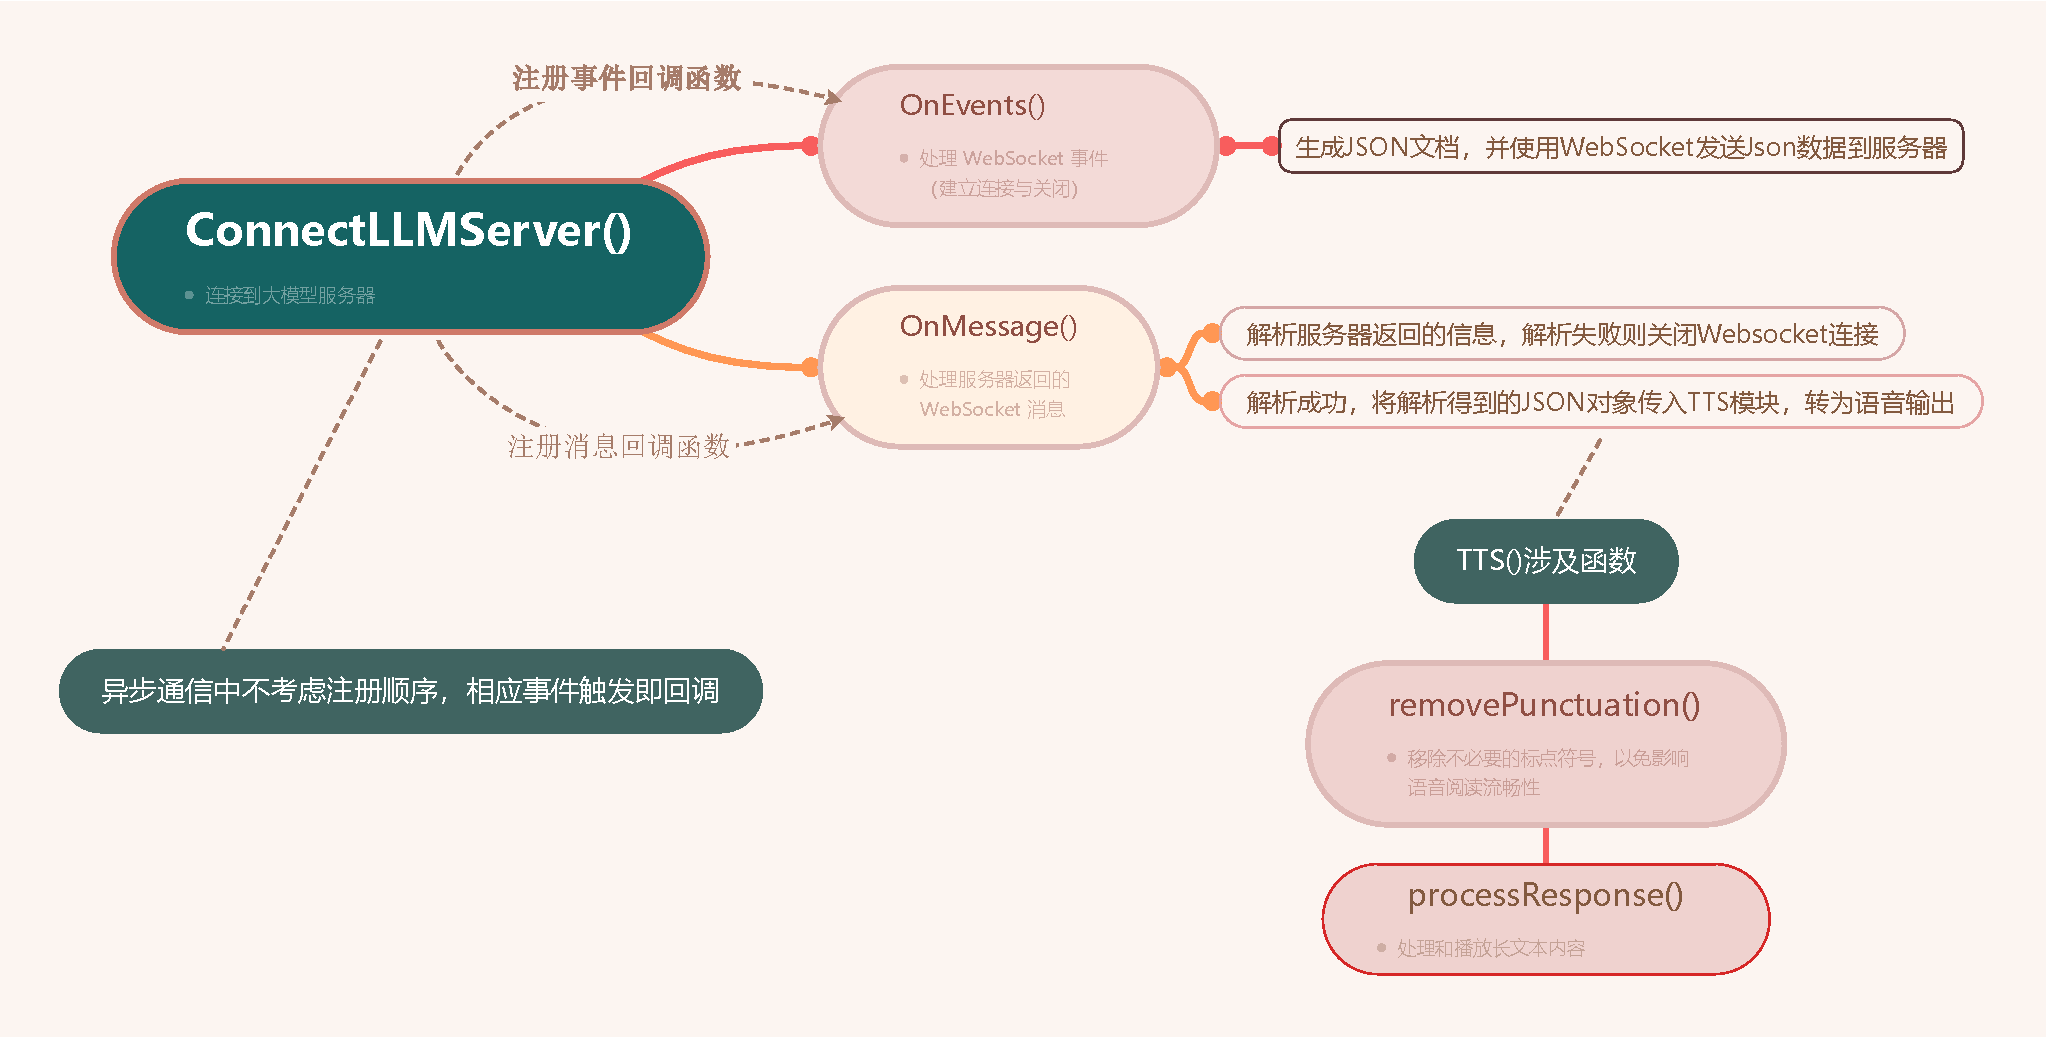
\includegraphics[width=0.9\textwidth]{../img/ConnectLLMServer.pdf}
    \caption{LLM与TTS交互的流程及实现}
    \label{fig:ConnectLLMServer}
\end{figure}